\documentclass[11pt]{article}
\usepackage[margin=1in]{geometry}
\usepackage[slantedGreek]{mathpazo}
\usepackage[pdftex]{graphicx}
\usepackage{amsmath,amssymb,amsfonts}
\usepackage{booktabs}
\usepackage{float}
\usepackage{caption}
\usepackage[numbers,sort&compress]{natbib}
\usepackage{hyperref}
\hypersetup{colorlinks=true,linkcolor=black,citecolor=black,urlcolor=blue}
\bibliographystyle{plainnat}

\graphicspath{{figures/}{gen/}}
% AUTO-GENERATED by tools/make_numbers.py -- do not edit.
\newcommand{\cpDirClearLoSpan}{81}
\newcommand{\cpDirSevereLoSpan}{56}
\newcommand{\cpDirClearHiSpan}{4}
\newcommand{\cpSupClearHiSpan}{31}
\newcommand{\cpSupLoSpanMin}{71}
\newcommand{\cpSupLoSpanMax}{78}
\newcommand{\cpSupLoSpanSpread}{7}
\newcommand{\cpStarLoSpan}{1}
\newcommand{\cpStarHiSpan}{0}
\newcommand{\cpDeltaMax}{34}
\newcommand{\cpDeltaHiSpanClear}{27}
\newcommand{\ucThreeSuccFast}{22}
\newcommand{\ucThreeSuccCover}{99}
\newcommand{\ucThreeLossFast}{6.1}
\newcommand{\ucThreeLossCover}{0.7}
\newcommand{\ucThreeTimeFast}{468}
\newcommand{\ucThreeTimeCover}{1082}
\newcommand{\ucThreeTempoRatio}{2.3}
\newcommand{\ucFiveSwarmMax}{8}
\newcommand{\ucFiveSuccBlind}{2}
\newcommand{\ucFiveSuccBestClear}{80}
\newcommand{\ucFiveSuccBestSevere}{52}
\newcommand{\ucFiveCovBlind}{0.01}
\newcommand{\ucFiveCovBestClear}{0.79}
\newcommand{\ucFiveCovBestSevere}{0.39}
\newcommand{\ucFiveSuccMidClear}{56}
\newcommand{\ucFiveSuccMidSevere}{28}
\newcommand{\lanchMaxErr}{9.1}
\newcommand{\beliefNRep}{24}
\newcommand{\beliefBaseLoss}{6.3}
\newcommand{\beliefCleanLoss}{6.4}
\newcommand{\beliefDecoyLoss}{3.8}
\newcommand{\beliefJamLoss}{5.2}
\newcommand{\nRep}{300}


\newcommand{\sandtable}{\textsc{SandTable}}
\captionsetup{font=small,labelfont=bf}

\title{\sandtable{}: A Fast Mission-Level Testbed for\\
Human-Machine Teaming Experiments Under Contested Communications}
\author{Vadim Sokolov\\
\small Department of Systems Engineering and Operations Research\\[-2pt]
\small George Mason University\\[-2pt]
\small \texttt{vsokolov@gmu.edu}}
\date{\today}

\begin{document}
\maketitle

\begin{abstract}
Designing human-machine teams for contested ground operations requires comparing many
combinations of control modality, formation, and autonomy against uncertain communications and
electronic warfare (EW). High-fidelity engines such as the Army's Government-furnished
\emph{ProjectGL} render each mission at or near real time, which is too slow for the thousands of
Monte-Carlo replications an optimizer or a design-of-experiments sweep needs. We present
\sandtable{}, a lightweight, pure-Python, mission-level simulator that stands in for that engine
inside the experiment inner loop. A mission is a pure function of scenario, seed, and design
parameters, so runs are reproducible, cacheable, and trivially parallel; a full mission of up to
1800 time steps completes in about a tenth of a second on one CPU core. \sandtable{} plugs into a
Bayesian-optimization and DOE orchestrator, and we drive \nRep{} replications per design across
147 designs (about 44,100 replications) on an HPC cluster. Its attrition kernel
reproduces Lanchester's square law to within \lanchMaxErr\%. Three studies yield decision-relevant
results. First, the direct-to-supervisory control optimum \emph{moves}: at a low span of control
(one operator to two assets) direct control wins only when communications are clear, while at high
span (one to eight) on-platform autonomy wins even in the clear, by up to \cpDeltaMax{}~percentage
points. Second, route choice traces a clean speed-survivability frontier: a defilade route reaches
\ucThreeSuccCover\% mission success against \ucThreeSuccFast\% for a fast exposed corridor, at
\ucThreeTempoRatio$\times$ the time. Third, a recon swarm cueing near-blind shooters lifts success
from \ucFiveSuccBlind\% (no recon) to \ucFiveSuccBestClear\%, but jamming severs the
sensor-to-shooter chain and cuts that to \ucFiveSuccBestSevere\%. \sandtable{} is offered as the
fast inner-loop companion to ProjectGL for Army mission engineering.
\end{abstract}

\section{Introduction}
\label{sec:intro}

The U.S. Army's shift toward human-machine teams, dismounted squads working with robotic combat
vehicles, uncrewed aircraft, and sensor nodes, turns tactics into a design problem. A mission
engineer must decide how one operator's attention is divided across autonomous assets, whether
control should be direct or supervisory, which route a formation takes, and how large a recon
swarm should be, all under communications that an adversary actively degrades. Each of these is a
knob, and the knobs interact: the best control modality depends on the communications state, and
the value of a recon swarm depends on whether its picture survives jamming. Answering such
questions demands experiments that sweep the knobs and measure outcomes against an engineered
ground truth, not one-off demonstrations.

ProjectGL, the Army's Government-furnished simulation framework built on Unreal Engine, is the
authoritative environment for this work \citep{stanko2025projectgl}. It models vehicle dynamics,
sensing, and synthetic terrain at high fidelity and won a 2024 Army Modeling and Simulation award.
That fidelity is exactly what makes it unsuitable for the \emph{inner loop} of a design study:
each mission runs at or near real time, so a modest experiment of a few hundred design points, each
averaged over a few hundred stochastic replications, would take weeks of wall-clock time. Bayesian
optimization and sensitivity analysis need the objective evaluated thousands of times, quickly and
reproducibly. The fidelity that makes ProjectGL the right tool for crew-station development and
final validation makes it the wrong tool for searching a design space.

We resolve this with a two-tier workflow. A fast, low-fidelity, mission-level model searches the
design space and locates the decision-relevant regions; the high-fidelity engine then validates the
handful of designs that matter. This paper builds and exercises the fast tier. \sandtable{} is a
pure-Python simulator that keeps the mission-level effects that drive design decisions, movement
over trafficable terrain, probabilistic sensing and engagement, a two-tier command model, and a
communications/EW degradation ladder, while discarding the physics and rendering that dominate
high-fidelity cost. It follows the ``accurate enough, not high fidelity'' principle: the model is
kept only as detailed as it must be to produce the right \emph{ordering} of design alternatives.

A model built for a search loop must satisfy two properties that ordinary simulators often do not.
It must be a \emph{pure function} of its inputs, with no global or hidden state, so that a run is
reproducible from its seed, cacheable, and safe to evaluate in parallel; and it must carry an
\emph{engineered ground truth}, a known correct answer for each trial, so that outcomes are scored
against truth rather than against agreement with the model's own agents. \sandtable{} is designed
around both.

\paragraph{Contributions} This paper makes the following four contributions.
\begin{enumerate}
\item \sandtable{}, a fast, reproducible, pure-Python mission-level simulator whose
\texttt{run\_mission} contract is a pure function of (scenario, seed, parameters), wired into a
Bayesian-optimization/DOE orchestrator and an HPC batch runner as the fast inner-loop companion to
ProjectGL (Section~\ref{sec:model}).
\item A control-modality model, direct human-in-the-loop versus supervisory autonomy, coupled to
span of control and a C0--C5 communications/EW ladder, that reproduces a \emph{moving optimum}: the
communications level at which autonomy overtakes human control falls as span rises
(Section~\ref{subsec:centerpiece}).
\item Three decision-relevant findings for Army human-machine teaming, the moving control optimum,
the speed-survivability frontier of route choice (Section~\ref{subsec:uc3}), and the EW-induced
collapse of a sensor-to-shooter chain (Section~\ref{subsec:uc5}), each generated from
\nRep{}-replication Monte-Carlo studies with confidence intervals.
\item An analytic validation: \sandtable{}'s emergent attrition matches Lanchester's square law to
within \lanchMaxErr\%, with the residual explained by known discretization effects
(Section~\ref{subsec:validation}).
\end{enumerate}

\section{Background and Related Work}
\label{sec:related}

\paragraph{Mission engineering and ProjectGL.} Mission engineering analyzes how systems combine to
accomplish a mission and traces measures of effectiveness back to design choices
\citep{raz2024mission}. ProjectGL provides the Army's shared, modular basis for such analysis in the
ground domain \citep{stanko2025projectgl}. \sandtable{} does not replace it; it occupies the fast
end of a fidelity spectrum, producing the response surfaces that tell an engineer which designs are
worth running at high fidelity.

\paragraph{Human-machine teaming and supervisory control.} The distinction between direct and
supervisory control dates to early telerobotics \citep{sheridan1978supervisory}, and the limits of
a single operator's situation awareness \citep{endsley1995awareness} and attention set how many
assets that operator can effectively command. Operator-capacity models estimate this span from
task timing \citep{cummings2007capacity}, and reviews of human-agent teaming and multi-robot
supervision catalog the resulting interface and workload issues
\citep{chen2014teaming,chen2011supervisory}. \sandtable{} abstracts these findings into a
tractable queueing model of operator attention (Section~\ref{sec:model}) whose behavior we then
map across the span-by-communications design space. For uncrewed-aircraft swarms specifically, a
meta-analysis of swarm-management interfaces documents how operator performance degrades as swarm
size and tempo grow \citep{hocraffer2017meta}, which motivates our sensor-swarm study.

\paragraph{Agent-based combat simulation.} Low-fidelity, effect-based combat models have a long
lineage. Flocking rules generate formation movement from local interactions
\citep{reynolds1987flocks}; operation-time agent frameworks schedule swarm tasks against a mission
clock \citep{wei2013operation}; and general agent-based modeling frameworks such as Mesa
\citep{masad2015mesa} popularized the pattern we follow, though for a tight optimization loop we use
a bespoke vectorized state representation rather than per-agent Python objects. A recurring lesson
in this literature is to validate an emergent model against a closed-form law; we adopt Lanchester's
square law \citep{kress2020lanchester} for that purpose.

\paragraph{Design of experiments and optimization.} The studies here are batch DOE sweeps; the same
plumbing supports Bayesian optimization via Monte-Carlo acquisition functions
\citep{balandat2020botorch} when a design space is too large to grid. The simulator core is built on
vectorized array programming \citep{harris2020numpy}.

\section{The \sandtable{} Model}
\label{sec:model}

\subsection{Design contract}
The top-level interface is a pure function
\[
\texttt{run\_mission}(\text{scenario}, \text{seed}, \text{params}) \;\rightarrow\; \text{metrics},
\]
with no module-level state, no global random number generator, and no file or wall-clock access in
the hot path. A companion \texttt{evaluate} averages the metrics over $n$ seeded replications. This
boundary is what makes a run reproducible from its seed, cacheable, and safe to evaluate
concurrently, and it is what lets the optimizer treat the simulator as a black-box objective. All
randomness is drawn from a single generator seeded per replication, so identical seeds reproduce
identical metrics bit for bit, and matched seed blocks across paired studies implement common random
numbers for low-variance comparison.

\subsection{State and time}
Entities (ground vehicles, uncrewed aircraft, sensor and command nodes, and defenders) are stored
as a structure of arrays: position, heading, health, sensor and weapon parameters, and side live in
parallel NumPy arrays rather than in per-agent objects \citep{harris2020numpy}. The mission advances
on a fixed time step (1~s here). Each step updates, in order, command tasking, planning, motion,
sensing, and engagement. This vectorized design runs a full mission of up to 1800 steps in roughly
0.1~s on a single core, about 7 to 11 replications per second depending on scenario, so
the 44,100 replications behind this paper are a few core-hours, trivially parallel across a
cluster.

\subsection{Movement, sensing, and engagement}
Ground platforms follow a unicycle kinematic model, with speed capped by a precomputed
trafficability field, and steer along a lane chosen by a \texttt{route\_bias} parameter that
interpolates between a fast exposed corridor and a slower covered route. Sensing is a
range-limited detection draw feeding a per-side shared picture, so recon aircraft can cue ground
shooters that have not detected a threat themselves. Engagement is aimed fire: every living shooter
engages its nearest detected enemy within weapon range, and a kill is a Bernoulli draw with
probability $p_k(1-c)$, where $c$ is the target's terrain cover. Both sides resolve against the
same pre-step state so there is no ordering bias. This effect-based abstraction is deliberately
coarse; Section~\ref{subsec:validation} shows it still obeys the right aggregate law.

\subsection{Command model: direct versus supervisory}
The command layer is where the human-machine teaming questions live. In \emph{supervisory} mode
each asset runs on-platform autonomy at a steady control quality $q_{\text{auto}}$, independent of
communications. In \emph{direct} mode a single human operator issues commands over the modeled
communications link: a well-served asset acts at a high quality $q_{\text{operator}}$, but commands
incur a round-trip latency and can be dropped, and while an asset waits it acts at a degraded stall
quality. Crucially, the operator is a single server shared across all supervised assets. Attention
dilutes with span: the effective operator quality is
\[
q_{\text{operator}}^{\text{eff}} = q_{\text{auto}} + \big(q_{\text{operator}} - q_{\text{auto}}\big)\,
\min\!\Big(1, \tfrac{\kappa}{n}\Big),
\]
where $n$ is the number of supervised assets and $\kappa$ the operator's service capacity. Below
capacity the operator adds full value; above it, requests queue and the human-in-the-loop advantage
erodes. Control quality feeds engagement (a well-controlled shooter is more effective; a poorly
controlled or stalled asset exposes itself), so the abstract quality translates into mission
outcomes. This model, an operator as a capacity-limited server whose value is gated by both span
and link quality, is the mechanism behind the moving optimum of Section~\ref{subsec:centerpiece},
and it is grounded in the operator-capacity and supervisory-control literature
\citep{cummings2007capacity,chen2011supervisory}.

\subsection{Communications and EW ladder}
A single \texttt{comms\_level} parameter indexes a C0--C5 degradation ladder, from clear (C0) to
severe (C5), that raises tasking latency and message-drop probability and thins the shared picture
by dropping relayed contacts. Because supervisory autonomy does not depend on the link while direct
control does, the ladder is the axis along which the two modalities separate.

\subsection{Engineered ground truth}
Every scenario carries a correct answer for the trial (which threats exist, which route survives,
what outcome a design should produce), and every agent exposes dial-able error and confidence. This
is what lets a study score a design against truth rather than against agreement with the model's own
agents, and it is a prerequisite for the pattern-detection objectives the broader program pursues.

\section{Experimental Setup}
\label{sec:setup}

We study three scenarios drawn from the program's use-case library. UC-3 (route choice) sweeps a
ground formation's \texttt{route\_bias} from a fast corridor to a covered defilade route. The
centerpiece crosses control modality (direct, supervisory) with span of control (one operator to
$\{2,3,4,5,6,8\}$ assets) and the C0--C5 communications ladder, in a fair fight where red strength
scales with blue. UC-5 (sensor swarm) sweeps recon swarm size ($0$ to $\ucFiveSwarmMax{}$ aircraft)
against the C0--C5 ladder, with the swarm cueing near-blind ground shooters against a defense in
depth.

Each design point is averaged over \nRep{} Monte-Carlo replications. Seeds are derived so that
matching cells across the paired direct and supervisory studies share seed blocks, giving common
random numbers for the paired comparison. Studies are declared as YAML and executed by the DOE
orchestrator through its SLURM runner on the GMU Hopper cluster: one batch job per design point,
each running its \nRep{} replications. Reported outcomes are mission success rate (fraction of
replications meeting the objective), attrition (mean losses per side), time to objective, and, for
UC-5, detection coverage (the time-averaged fraction of the live threat force held on the shared
picture). Success-rate confidence intervals are the normal approximation
$1.96\sqrt{p(1-p)/\nRep{}}$, about 6~percentage points at $p=0.5$.

All numbers and tables in this paper are generated from the study outputs by a single script and
inlined, so every value traces to code and data.

\section{Results}
\label{sec:results}

\subsection{Validation against Lanchester's square law}
\label{subsec:validation}

Before drawing design conclusions we check that the attrition kernel obeys a recognized combat law.
\sandtable{} resolves fire as aimed fire, so when fire is distributed the kill rate on a side is
proportional to the number of opposing shooters, which is the hypothesis of Lanchester's square law
\citep{kress2020lanchester}. For equal effectiveness the stronger side annihilates the weaker and
its survivors are $\sqrt{B_0^2 - R_0^2}$. We isolate the kernel (no movement, no cover, mutual
detection, forces intermixed so fire distributes) and compare the Monte-Carlo mean survivors to that
closed form (Table~\ref{tab:lanchester}). Agreement is within \lanchMaxErr\%, biased slightly low.
The bias is expected and conservative: simultaneous discrete-time resolution lets a unit about to
die still return fire (an effect that vanishes as the per-step kill probability shrinks), and
nearest-target assignment produces occasional overkill. A low-fidelity model reproducing the square
law to within a few percent is the defensibility check this class of model calls for.

\begin{table}[H]
\centering
\caption{Attrition kernel versus Lanchester's square law. Mean surviving stronger-side units over
600 replications per duel; ``square law'' is $\sqrt{B_0^2-R_0^2}$.}
\label{tab:lanchester}
\begin{tabular}{rrrrr}
\toprule
$B_0$ & $R_0$ & sim $B$ surv. & Lanchester $B$ & rel. err. \\
\midrule
10 & 6 & 7.49 & 8.00 & -6.4\% \\
12 & 8 & 8.13 & 8.94 & -9.1\% \\
16 & 10 & 11.79 & 12.49 & -5.6\% \\
20 & 12 & 15.42 & 16.00 & -3.6\% \\
20 & 16 & 11.02 & 12.00 & -8.2\% \\
30 & 20 & 21.75 & 22.36 & -2.7\% \\
\bottomrule
\end{tabular}

\end{table}

\subsection{Route choice: the speed-survivability frontier}
\label{subsec:uc3}

UC-3 asks how a ground formation should trade tempo against exposure. Figure~\ref{fig:uc3} and
Table~\ref{tab:uc3} sweep the route from a fast exposed corridor (\texttt{route\_bias}~$=0$) to a
covered defilade route (\texttt{route\_bias}~$=1$). The trade is clean and monotone. The fast
corridor reaches the objective in \ucThreeTimeFast{}~s but succeeds only \ucThreeSuccFast\% of the
time and loses \ucThreeLossFast{} of eight vehicles; the covered route succeeds \ucThreeSuccCover\%
of the time and loses \ucThreeLossCover{}, at the cost of \ucThreeTimeCover{}~s, roughly
\ucThreeTempoRatio$\times$ longer. Panel~(b) plots the resulting frontier: there is no free lunch,
only a quantified exchange rate between minutes and casualties that a mission engineer can price
against the tactical situation. That the model produces a smooth, well-ordered frontier rather than
noise is the sensitivity property a search loop requires.

\begin{figure}[H]
\centering
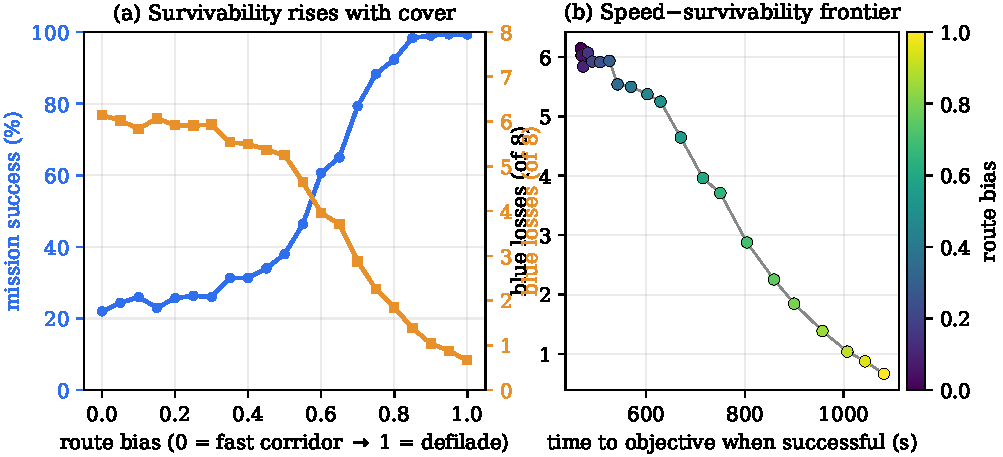
\includegraphics[width=\textwidth]{uc3_frontier.pdf}
\caption{UC-3 route choice. (a) Mission success rises and attrition falls as the route moves from
the fast corridor toward defilade cover. (b) The speed-survivability frontier: time to objective
against blue losses, colored by route bias. Bands and markers are means over \nRep{} replications.}
\label{fig:uc3}
\end{figure}

\begin{table}[H]
\centering
\caption{UC-3 route choice, selected route-bias points (means over \nRep{} replications).}
\label{tab:uc3}
\begin{tabular}{rrrrr}
\toprule
route bias & success (\%) & blue losses (of 8) & red losses (of 6) & $t_{\text{obj}}$ (s) \\
\midrule
0.00 & 22 & 6.1 & 1.9 & 468 \\
0.25 & 26 & 5.9 & 2.1 & 507 \\
0.50 & 38 & 5.2 & 2.6 & 629 \\
0.75 & 88 & 2.3 & 4.1 & 859 \\
1.00 & 99 & 0.7 & 4.7 & 1082 \\
\bottomrule
\end{tabular}

\end{table}

\subsection{The moving optimum: span of control under EW}
\label{subsec:centerpiece}

The centerpiece study crosses control modality with span of control and the communications ladder.
Figure~\ref{fig:cp_curves} shows the mechanism directly. Supervisory autonomy is nearly
communications-invariant: at a span of one operator to two assets its success stays between
\cpSupLoSpanMin\% and \cpSupLoSpanMax\% across the entire ladder (a spread of \cpSupLoSpanSpread{}
percentage points). Direct control degrades along two axes at once. It falls with communications,
from \cpDirClearLoSpan\% at C0 to \cpDirSevereLoSpan\% at C5 for the one-to-two span, and it falls
with span, because the single operator saturates: at one-to-eight, direct control is already floored
at \cpDirClearHiSpan\% even in clear communications, against \cpSupClearHiSpan\% for supervisory.

Figure~\ref{fig:cp_phase} collapses the full design space into a single decision aid. Each cell is
the supervisory-minus-direct success difference; blue cells (bottom-left, low span and clear
communications) are where a human in the loop wins, red cells everywhere else are where on-platform
autonomy wins, and the black contour is the crossover. The optimum \emph{moves}. At the smallest
span the crossover sits at C$\cpStarLoSpan{}$: direct control is competitive only while
communications are near-clear. As span grows the crossover slides left until, at one-to-eight,
supervisory autonomy dominates at every communications level (crossover C$\cpStarHiSpan{}$), by as
much as \cpDeltaMax{}~percentage points. The single most decision-relevant reading is the boundary
itself: the more assets one operator must supervise, the less communications degradation it takes
before control should be handed to the machines. Table~\ref{tab:centerpiece} gives the full grid.

\begin{figure}[H]
\centering
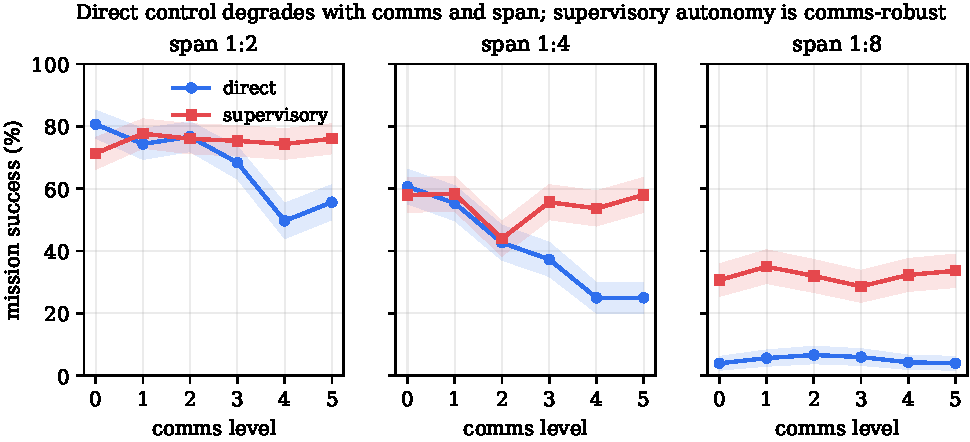
\includegraphics[width=\textwidth]{centerpiece_curves.pdf}
\caption{Mission success versus communications degradation for direct (blue) and supervisory (red)
control, at three spans of control. Direct control degrades with both communications and span;
supervisory autonomy is comms-robust. Bands are \nRep{}-replication binomial confidence intervals.}
\label{fig:cp_curves}
\end{figure}

\begin{figure}[H]
\centering
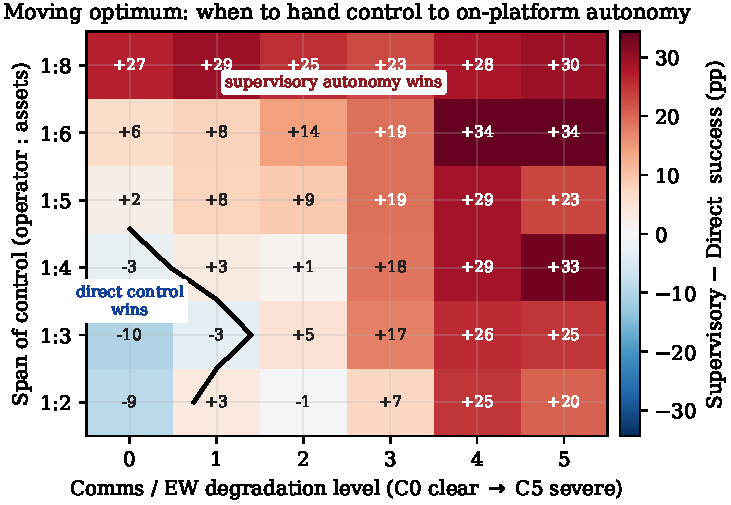
\includegraphics[width=0.82\textwidth]{centerpiece_phase.pdf}
\caption{The moving optimum. Cell value is supervisory-minus-direct mission success (percentage
points) over span of control and communications degradation. The black contour marks the crossover;
it sweeps from the low-span, clear-communications corner, so more assets or worse communications
both push the decision toward autonomy.}
\label{fig:cp_phase}
\end{figure}

\begin{table}[H]
\centering
\caption{Centerpiece: supervisory-minus-direct mission success (percentage points) over span of
control (rows) and communications level (columns). Positive favors supervisory autonomy.}
\label{tab:centerpiece}
\begin{tabular}{rrrrrrr}
\toprule
span & C0 & C1 & C2 & C3 & C4 & C5 \\
\midrule
1:2 & -9 & +3 & -1 & +7 & +25 & +20 \\
1:3 & -10 & -3 & +5 & +17 & +26 & +25 \\
1:4 & -3 & +3 & +1 & +18 & +29 & +33 \\
1:5 & +2 & +8 & +9 & +19 & +29 & +23 \\
1:6 & +6 & +8 & +14 & +19 & +34 & +34 \\
1:8 & +27 & +29 & +25 & +23 & +28 & +30 \\
\bottomrule
\end{tabular}

\end{table}

\subsection{Sensor swarm under electronic warfare}
\label{subsec:uc5}

UC-5 pairs a recon swarm with near-blind ground shooters against a defense in depth, then jams the
link. Figure~\ref{fig:uc5} and Table~\ref{tab:uc5} give the result. With no recon the shooters
cannot see the threats that out-range them and the assault fails, succeeding only
\ucFiveSuccBlind\% of the time. Adding aircraft builds detection coverage with a clear threshold:
coverage climbs steeply until the swarm is large enough to blanket the depth of the defense (near
\ucFiveCovBestClear{} at the largest swarm in clear conditions) and mission success rises with it,
to \ucFiveSuccBestClear\%. The sensor-to-shooter chain is the whole story: recon is what lets blind
shooters engage, and swarm size buys the coverage that cues them.

Electronic warfare breaks that chain. As jamming intensifies it thins the shared picture, and both
coverage and success collapse toward the no-recon baseline at every swarm size. At the largest swarm,
success falls from \ucFiveSuccBestClear\% in clear conditions to \ucFiveSuccBestSevere\% under severe
EW, and coverage from \ucFiveCovBestClear{} to \ucFiveCovBestSevere{}; a mid-sized swarm collapses
from \ucFiveSuccMidClear\% to \ucFiveSuccMidSevere\%. The design implication is that swarm size and
communications resilience are complements, not substitutes: buying more aircraft raises the ceiling
in clear conditions but does not protect the picture once the link is contested.

\begin{figure}[H]
\centering
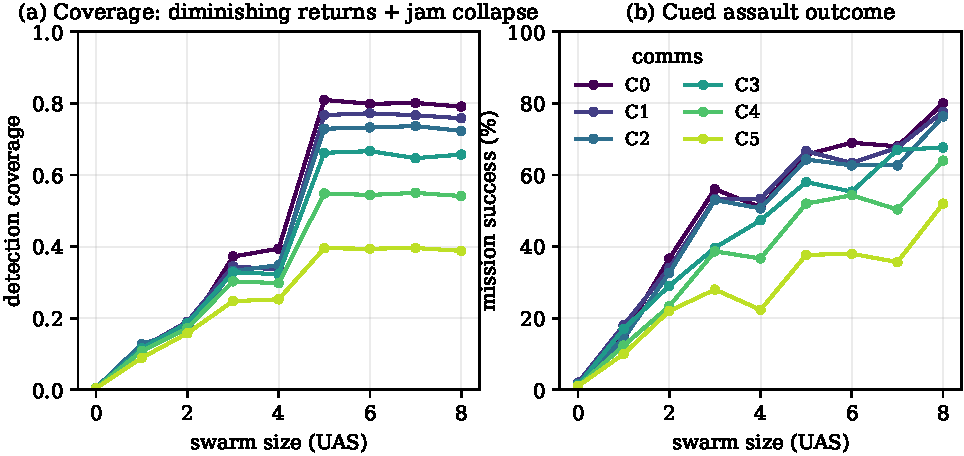
\includegraphics[width=\textwidth]{uc5_swarm_jam.pdf}
\caption{UC-5 sensor swarm under EW. (a) Detection coverage rises with swarm size, with a threshold
where the swarm blankets the defense in depth, then collapses as jamming (C0 clear to C5 severe)
thins the shared picture. (b) Cued mission success tracks coverage and falls with jamming at every
swarm size. Means over \nRep{} replications.}
\label{fig:uc5}
\end{figure}

\begin{table}[H]
\centering
\caption{UC-5 detection coverage (cov) and mission success (succ, \%) by swarm size and
communications level, means over \nRep{} replications.}
\label{tab:uc5}
\begin{tabular}{rrrrrrr}
\toprule
 & \multicolumn{2}{c}{C0} & \multicolumn{2}{c}{C3} & \multicolumn{2}{c}{C5} \\
\cmidrule(lr){2-3} \cmidrule(lr){4-5} \cmidrule(lr){6-7}
swarm & cov & succ & cov & succ & cov & succ \\
\midrule
0 & 0.01 & 2 & 0.00 & 1 & 0.00 & 1 \\
1 & 0.12 & 15 & 0.12 & 17 & 0.09 & 10 \\
2 & 0.17 & 37 & 0.19 & 29 & 0.16 & 22 \\
3 & 0.37 & 56 & 0.33 & 40 & 0.25 & 28 \\
4 & 0.39 & 51 & 0.32 & 47 & 0.25 & 22 \\
5 & 0.81 & 66 & 0.66 & 58 & 0.40 & 38 \\
6 & 0.80 & 69 & 0.67 & 55 & 0.39 & 38 \\
7 & 0.80 & 68 & 0.65 & 67 & 0.40 & 36 \\
8 & 0.79 & 80 & 0.66 & 68 & 0.39 & 52 \\
\bottomrule
\end{tabular}

\end{table}

\section{Discussion}
\label{sec:discussion}

The three studies share a structure that is useful to name. In each, the best design is not fixed
but \emph{contingent} on the contested-conditions axis, and \sandtable{} locates where the
contingency flips. Route choice prices tempo against survivability so a planner can pick a point on
the frontier to match the mission. The centerpiece turns span of control and communications state
into a single rule: hand control to autonomy sooner as either span or degradation grows, and the
phase diagram says exactly when. The swarm study shows that sensing capacity and link resilience
must be bought together, because EW attacks the chain that connects them. None of these is a
statement about one design; each is a map of how the right design moves as conditions change, which
is what mission engineering needs.

Methodologically, the results argue for the two-tier workflow. \sandtable{} ran 44,100
replications in a few core-hours and returned smooth, well-ordered response surfaces with tight
confidence intervals, precisely the regions and boundaries a high-fidelity ProjectGL study should
then confirm. The fast tier is not a replacement for fidelity; it is what makes fidelity affordable,
by spending the expensive engine only on the designs the cheap one has flagged.

\section{Limitations}
\label{sec:limitations}

\sandtable{} is deliberately low-fidelity, and its conclusions inherit that. Movement is 2.5D
kinematic, not physics-based; sensing and engagement are effect-based draws, not signal or
signature models; terrain is a scalar trafficability-and-cover field, not a rendered environment;
and line of sight is a flat-terrain stub. The command model is a capacity-limited-server
abstraction of operator attention, calibrated to the qualitative findings of the supervisory-control
literature rather than to human-subject data. The absolute success rates should therefore be read as
comparative, not predictive: the value is in the \emph{ordering} of designs and the \emph{location}
of crossovers, which is what a search loop consumes, not in any single percentage. The moving
optimum's exact crossover cells near the contour are within Monte-Carlo noise, so the robust claim is
the direction of the boundary, not its precise cell. The Lanchester check validates the aggregate
attrition law but not the spatial or command dynamics, which is why the intended role of the model is
to feed, not replace, high-fidelity validation.

\section{Conclusion}
\label{sec:conclusion}

We built \sandtable{}, a fast, reproducible, pure-Python mission-level testbed, as the inner-loop
companion to the Army's high-fidelity ProjectGL, and used it to produce three decision-relevant
maps for human-machine teaming under contested communications: a moving direct-to-supervisory
control optimum, a speed-survivability frontier for route choice, and the EW-induced collapse of a
sensor-to-shooter chain. The tool obeys a recognized attrition law, runs a full mission in about a
tenth of a second, and plugs directly into a Bayesian-optimization and DOE orchestrator, so the
next step is to search these design spaces with optimization rather than grids, and to confirm the
flagged designs in ProjectGL.

\section*{Acknowledgments}
This work was performed under the VIPR-GS FP6111 program (U.S. Army GVSC, via the Clemson-led
Army-Clemson Research Alliance). All work reported here is unclassified. Computation used the GMU
Hopper HPC cluster.

\bibliography{ref}

\end{document}
